% Figure: Layered Post-Infectious Pathogenesis — Five-Layer Temporal Cascade

\begin{figure}[htbp]
\centering
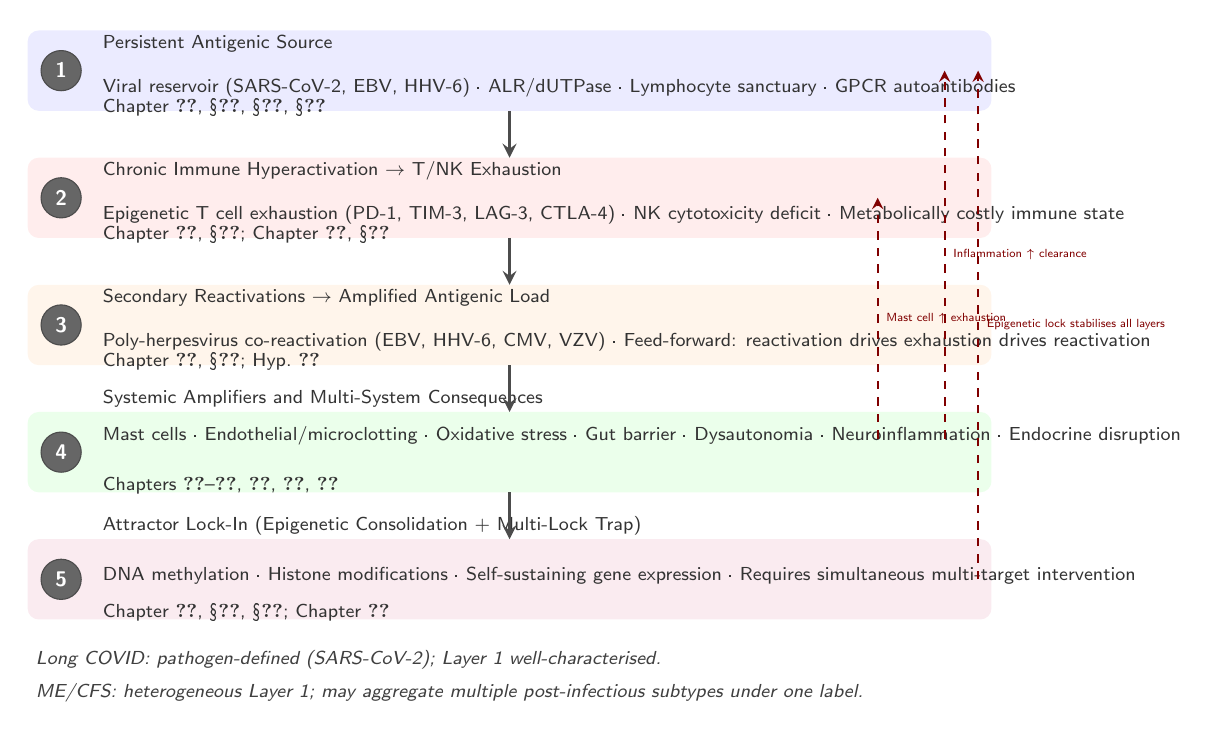
\begin{tikzpicture}[
    scale=0.85, every node/.style={scale=0.85},
    layerbox/.style={
      rectangle, draw=gray!60!black, thick,
      rounded corners=4pt, minimum width=13.5cm, minimum height=1.2cm,
      inner sep=0.25cm, align=left, font=\sffamily\small
    },
    layerbg/.style={
      rectangle, rounded corners=4pt, minimum width=13.5cm, minimum height=1.2cm,
    },
    layernum/.style={
      circle, draw=gray!60!black, fill=gray!80!black, text=white,
      minimum size=0.6cm, inner sep=0pt, font=\sffamily\bfseries\small
    },
    labeltext/.style={
      font=\sffamily\footnotesize, text=gray!40!black, anchor=west
    },
    arr/.style={-stealth, thick, gray!60!black},
    feedback/.style={-stealth, thick, red!50!black, dashed},
    cola/.style={fill=blue!8},
    colb/.style={fill=red!7},
    colc/.style={fill=orange!8},
    cold/.style={fill=green!8},
    cole/.style={fill=purple!8},
]

% ===== LAYER 1: Persistent Antigenic Source =====
\fill[blue!8, rounded corners=4pt] (-7.2, 3.6) rectangle (7.2, 2.4);
\node[layernum] (n1) at (-6.7, 3.0) {1};
\node[labeltext] at (-6.2, 3.4) {Persistent Antigenic Source};
\node[labeltext] at (-6.2, 2.75) {\footnotesize Viral reservoir (SARS-CoV-2, EBV, HHV-6) · ALR/dUTPase · Lymphocyte sanctuary · GPCR autoantibodies};
\node[labeltext] at (-6.2, 2.45) {\footnotesize Chapter~\ref{ch:immune-dysfunction}, \S\ref{sec:abortive-lytic}, \S\ref{sec:poly-herpesvirus}, \S\ref{sec:root-gpcr}};

% ===== LAYER 2: Chronic Immune Activation → Exhaustion =====
\fill[red!7, rounded corners=4pt] (-7.2, 1.7) rectangle (7.2, 0.5);
\node[layernum] (n2) at (-6.7, 1.1) {2};
\node[labeltext] at (-6.2, 1.5) {Chronic Immune Hyperactivation $\rightarrow$ T/NK Exhaustion};
\node[labeltext] at (-6.2, 0.85) {\footnotesize Epigenetic T cell exhaustion (PD-1, TIM-3, LAG-3, CTLA-4) · NK cytotoxicity deficit · Metabolically costly immune state};
\node[labeltext] at (-6.2, 0.55) {\footnotesize Chapter~\ref{ch:immune-dysfunction}, \S\ref{subsec:pembrolizumab}; Chapter~\ref{ch:disease-course}, \S\ref{hyp:immune-exhaustion-timeline}};

% ===== LAYER 3: Secondary Reactivations =====
\fill[orange!8, rounded corners=4pt] (-7.2, -0.2) rectangle (7.2, -1.4);
\node[layernum] (n3) at (-6.7, -0.8) {3};
\node[labeltext] at (-6.2, -0.4) {Secondary Reactivations $\rightarrow$ Amplified Antigenic Load};
\node[labeltext] at (-6.2, -1.05) {\footnotesize Poly-herpesvirus co-reactivation (EBV, HHV-6, CMV, VZV) · Feed-forward: reactivation drives exhaustion drives reactivation};
\node[labeltext] at (-6.2, -1.35) {\footnotesize Chapter~\ref{ch:immune-dysfunction}, \S\ref{sec:poly-herpesvirus}; Hyp.~\ref{hyp:viral-reactivation-bidirectional}};

% ===== LAYER 4: Systemic Amplifiers =====
\fill[green!8, rounded corners=4pt] (-7.2, -2.1) rectangle (7.2, -3.3);
\node[layernum] (n4) at (-6.7, -2.7) {4};
\node[labeltext] at (-6.2, -1.9) {Systemic Amplifiers and Multi-System Consequences};
\node[labeltext] at (-6.2, -2.45) {\footnotesize Mast cells · Endothelial/microclotting · Oxidative stress · Gut barrier · Dysautonomia · Neuroinflammation · Endocrine disruption};
\node[labeltext] at (-6.2, -3.2) {\footnotesize Chapters~\ref{ch:cardiovascular}--\ref{ch:gut-microbiome}, \ref{ch:neurological}, \ref{ch:endocrine}, \ref{ch:symptom-mechanisms}};

% ===== LAYER 5: Attractor Lock-In =====
\fill[purple!8, rounded corners=4pt] (-7.2, -4.0) rectangle (7.2, -5.2);
\node[layernum] (n5) at (-6.7, -4.6) {5};
\node[labeltext] at (-6.2, -3.8) {Attractor Lock-In (Epigenetic Consolidation + Multi-Lock Trap)};
\node[labeltext] at (-6.2, -4.55) {\footnotesize DNA methylation · Histone modifications · Self-sustaining gene expression · Requires simultaneous multi-target intervention};
\node[labeltext] at (-6.2, -5.1) {\footnotesize Chapter~\ref{ch:causal-hierarchy}, \S\ref{sec:amp-epigenetic}, \S\ref{sec:multi-lock-trap}; Chapter~\ref{ch:causal-hierarchy-formal}};

% ===== CAUSAL ARROWS (downward, Layer 1→2→3→4→5) =====
\draw[arr, line width=1.2pt] (0, 2.4) -- (0, 1.7);
\draw[arr, line width=1.2pt] (0, 0.5) -- (0, -0.2);
\draw[arr, line width=1.2pt] (0, -1.4) -- (0, -2.1);
\draw[arr, line width=1.2pt] (0, -3.3) -- (0, -4.0);

% ===== FEEDBACK ARROWS (upward, dashed) =====
% Layer 4 → Layer 1 (via inflammation and oxidative stress)
\draw[feedback] (6.5, -2.5) -- (6.5, 3.0)
  node[midway, right, font=\sffamily\tiny, text=red!50!black]
    {Inflammation $\uparrow$ clearance};

% Layer 4 → Layer 2 (via further immune impairment)
\draw[feedback] (5.5, -2.5) -- (5.5, 1.1)
  node[midway, right, font=\sffamily\tiny, text=red!50!black]
    {Mast cell $\uparrow$ exhaustion};

% Layer 5 → Layers 1--4 (epigenetic lock)
\draw[feedback] (7.0, -4.6) -- (7.0, 3.0)
  node[midway, right, font=\sffamily\tiny, text=red!50!black]
    {Epigenetic lock stabilises all layers};

% ===== LONG COVID / ME/CFS ANNOTATION =====
\node[font=\sffamily\footnotesize\itshape, text=gray!50!black, anchor=west]
  at (-7.2, -5.8)
  {Long COVID: pathogen-defined (SARS-CoV-2); Layer~1 well-characterised.};

\node[font=\sffamily\footnotesize\itshape, text=gray!50!black, anchor=west]
  at (-7.2, -6.3)
  {ME/CFS: heterogeneous Layer~1; may aggregate multiple post-infectious subtypes under one label.};

\end{tikzpicture}
\caption{The Layered Post-Infectious Pathogenesis model. Five layers form a temporal cascade from persistent antigenic source through immune exhaustion, secondary reactivations, systemic consequences, and attractor lock-in. Downward arrows represent causal progression; dashed red arrows represent feedback from later layers back to earlier ones, creating the self-sustaining cycles that define chronicity. The model applies to both Long COVID (SARS-CoV-2-defined Layer~1) and ME/CFS (heterogeneous Layer~1). Chapter citations indicate where each layer's mechanisms are documented in detail.}
\label{fig:layered-pathogenesis}
\end{figure}
